% SPDX-License-Identifier: CC-BY-SA-4.0
% Author: Matthieu Perrin
% Part: 
% Section: 
% Sub-section: 
% Frame: 

\begingroup

\SetKwFunction{Decider}{decider}
\SetKwFunction{Afficher}{Ecrire}
\SetKwData{Mot}{u}
\SetKwData{Symbols}{symbols}
\SetKwData{Final}{final\_state}
\SetKwData{Transition}{transitions}

\begin{frame}{Implémentation d'un automate déterministe complet}

  \tf[text, top=-1mm]{
    Un AFD $A = \left\langle \Sigma, Q, \{q_0\}, F, \rightarrow \right\rangle$ complet est modélisé par un enregistrement :\\
    
    \begin{description}
    \item[$\Symbols$ :] tableau de 256 entiers \hspace\fill \alert{classification des caractères}
    \item[$\Transition$ :] tableau de tableaux d'entiers \hspace\fill \alert{$q \xrightarrow{a} \Transition[a, q]$}
    \item[$\Final$ :] tableau de booléens \hspace\fill \alert{$q\in F \Leftrightarrow \Final[q]$}
    \end{description}
    Les états des entiers, l'état initial est $0$.
  }

  \tf[y=0mm]{\small
    \begin{algorithm}[H]
      \Fn{\Decider($u \in \Sigma^\star$, $A$ : AFN) : booléen}{
        $q \leftarrow 0$\;
        \Pour{$i$ de $1$ à $|u|$}{$q \leftarrow A.\Transition[A.\Symbols[u[i]], q]$}
        \Retourner $A.\Final[q]$\;
      }
    \end{algorithm}
  }

  \tf[width=30mm,y=2mm, x=35mm]{\small
    \structure{Complexité temporelle}\vspace{-1mm}
    $$\mathcal{O}(n)$$\\\vspace{-1mm}
    \structure{Complexité spatiale}\vspace{-1mm}
    $$\mathcal{O}(|Q| \times |\Sigma|)$$
  }  

  
  \tfExampleBlock[y=-15mm]{Exemple}{}

  \tf[x=-30mm, y=-29mm]{\footnotesize
    \begin{tikzpicture}[automaton, x=10mm, y=6mm]
      \node[state, initial left]   (0) at (0,2) {$0$}; 
      \node[state]            (1) at (2,2) {$1$}; 
      \node[state]            (2) at (2,0) {$2$}; 
      \node[state, accepting] (3) at (0,0) {$3$};
      \node[Fade, state]      (4) at (1,1) {$4$}; 
      
      \path (0) edge[bend left=3mm] node{a-z} (1);
      \path (1) edge[bend left=3mm] node{.}   (0);
      \path (1) edge                node{@}   (2);
      \path (2) edge[bend left=3mm] node{a-z} (3);
      \path (3) edge[bend left=3mm] node{.}   (2);
      \path (1) edge[loop right   ] node{a-z} (1);
      \path (3) edge[loop left    ] node{a-z} (3);
      
      \path[Fade] (0) edge             (4);
      \path[Fade] (1) edge             (4);
      \path[Fade] (2) edge             (4);
      \path[Fade] (3) edge             (4);
      \path[Fade] (4) edge[loop left]  (4);
    \end{tikzpicture}
  }

  \tf[x=25mm, y=-25mm]{
    $\begin{array}{@{\;}l@{\;}c@{\;}l@{\;}}
      \Symbols &\leftarrow&
      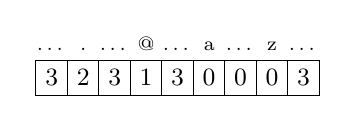
\begin{tikzpicture}[x=4mm, y=4mm, baseline=(center)]
        \coordinate (center) at (0,-1mm);
        \node[draw, rectangle, minimum width=4mm] (x) at (0,0) {\small 3};  \node[above] at (x.north) {\scriptsize \ldots}; 
        \node[draw, rectangle, minimum width=4mm] (x) at (1,0) {\small 2};  \node[above] at (x.north) {\scriptsize .};      
        \node[draw, rectangle, minimum width=4mm] (x) at (2,0) {\small 3};  \node[above] at (x.north) {\scriptsize \ldots}; 
        \node[draw, rectangle, minimum width=4mm] (x) at (3,0) {\small 1};  \node[above] at (x.north) {\scriptsize @};      
        \node[draw, rectangle, minimum width=4mm] (x) at (4,0) {\small 3};  \node[above] at (x.north) {\scriptsize \ldots}; 
        \node[draw, rectangle, minimum width=4mm] (x) at (5,0) {\small 0};  \node[above] at (x.north) {\scriptsize a};      
        \node[draw, rectangle, minimum width=4mm] (x) at (6,0) {\small 0};  \node[above] at (x.north) {\scriptsize \ldots}; 
        \node[draw, rectangle, minimum width=4mm] (x) at (7,0) {\small 0};  \node[above] at (x.north) {\scriptsize z};      
        \node[draw, rectangle, minimum width=4mm] (x) at (8,0) {\small 3};  \node[above] at (x.north) {\scriptsize \ldots}; 
      \end{tikzpicture}\\
      \Transition &\leftarrow&
      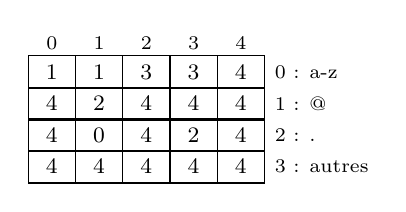
\begin{tikzpicture}[x=6mm, y=4mm, baseline=(center)]
        \coordinate (center) at (0,11mm);
        \node[draw, rectangle, minimum width=6mm, minimum height=4mm] (x) at (0,3) {\footnotesize 1}; \node[above] at ([yshift=-.5mm]x.north) {\scriptsize 0};
        \node[draw, rectangle, minimum width=6mm, minimum height=4mm] (x) at (1,3) {\footnotesize 1}; \node[above] at ([yshift=-.5mm]x.north) {\scriptsize 1};
        \node[draw, rectangle, minimum width=6mm, minimum height=4mm] (x) at (2,3) {\footnotesize 3}; \node[above] at ([yshift=-.5mm]x.north) {\scriptsize 2};
        \node[draw, rectangle, minimum width=6mm, minimum height=4mm] (x) at (3,3) {\footnotesize 3}; \node[above] at ([yshift=-.5mm]x.north) {\scriptsize 3};
        \node[draw, rectangle, minimum width=6mm, minimum height=4mm] (x) at (4,3) {\footnotesize 4}; \node[above] at ([yshift=-.5mm]x.north) {\scriptsize 4}; \node[right] at (x.east) {\scriptsize 0 : a-z};
        \node[draw, rectangle, minimum width=6mm, minimum height=4mm] (x) at (0,2) {\footnotesize 4}; 
        \node[draw, rectangle, minimum width=6mm, minimum height=4mm] (x) at (1,2) {\footnotesize 2}; 
        \node[draw, rectangle, minimum width=6mm, minimum height=4mm] (x) at (2,2) {\footnotesize 4}; 
        \node[draw, rectangle, minimum width=6mm, minimum height=4mm] (x) at (3,2) {\footnotesize 4}; 
        \node[draw, rectangle, minimum width=6mm, minimum height=4mm] (x) at (4,2) {\footnotesize 4}; \node[right] at (x.east) {\scriptsize 1 : @};
        \node[draw, rectangle, minimum width=6mm, minimum height=4mm] (x) at (0,1) {\footnotesize 4}; 
        \node[draw, rectangle, minimum width=6mm, minimum height=4mm] (x) at (1,1) {\footnotesize 0}; 
        \node[draw, rectangle, minimum width=6mm, minimum height=4mm] (x) at (2,1) {\footnotesize 4}; 
        \node[draw, rectangle, minimum width=6mm, minimum height=4mm] (x) at (3,1) {\footnotesize 2}; 
        \node[draw, rectangle, minimum width=6mm, minimum height=4mm] (x) at (4,1) {\footnotesize 4}; \node[right] at (x.east) {\scriptsize 2 : .};
        \node[draw, rectangle, minimum width=6mm, minimum height=4mm] (x) at (0,0) {\footnotesize 4}; 
        \node[draw, rectangle, minimum width=6mm, minimum height=4mm] (x) at (1,0) {\footnotesize 4}; 
        \node[draw, rectangle, minimum width=6mm, minimum height=4mm] (x) at (2,0) {\footnotesize 4}; 
        \node[draw, rectangle, minimum width=6mm, minimum height=4mm] (x) at (3,0) {\footnotesize 4}; 
        \node[draw, rectangle, minimum width=6mm, minimum height=4mm] (x) at (4,0) {\footnotesize 4}; \node[right] at (x.east) {\scriptsize 3 : autres};
      \end{tikzpicture}\vspace{.5mm}\\
      \Final &\leftarrow&
      
\begin{tikzpicture}[x=6mm, y=4mm, baseline=(center)]
        \coordinate (center) at (0,-1mm);
        \node[draw, rectangle, minimum width=6mm] (x) at (0,0) {\tiny\Faux}; 
        \node[draw, rectangle, minimum width=6mm] (x) at (1,0) {\tiny\Faux};     
        \node[draw, rectangle, minimum width=6mm] (x) at (2,0) {\tiny\Faux}; 
        \node[draw, rectangle, minimum width=6mm] (x) at (3,0) {\tiny\Vrai};     
        \node[draw, rectangle, minimum width=6mm] (x) at (4,0) {\tiny\Faux}; 
      \end{tikzpicture}\\
    \end{array}
    $
  }

\end{frame}

\endgroup
